\documentclass{article} % For LaTeX2e
\usepackage{nips13submit_e,times}
\usepackage{hyperref}
\usepackage{url}
\usepackage{amsmath}
\usepackage{color}
\definecolor{Ao}{rgb}{0.0, 0.5, 0.0}
\definecolor{bostonuniversityred}{rgb}{0.8, 0.0, 0.0}

\usepackage{array}
\newcolumntype{P}[1]{>{\centering\arraybackslash}p{#1}}
\usepackage[toc,page]{appendix}
\usepackage{graphicx}
\graphicspath{{../../analysis/}}

\usepackage{float}
\restylefloat{table}
%\documentstyle[nips13submit_09,times,art10]{article} % For LaTeX 2.09

\title{Flame Wars: Automatic Insult Detection}


\author{
Sasha Sax \thanks{ sashasax.com } \\
Department of Computer Science\\
Stanford University\\
\texttt{sax@cs.stanford.edu}
}

% The \author macro works with any number of authors. There are two commands
% used to separate the names and addresses of multiple authors: \And and \AND.
%
% Using \And between authors leaves it to \LaTeX{} to determine where to break
% the lines. Using \AND forces a linebreak at that point. So, if \LaTeX{}
% puts 3 of 4 authors names on the first line, and the last on the second
% line, try using \AND instead of \And before the third author name.

\newcommand{\fix}{\marginpar{FIX}}
\newcommand{\new}{\marginpar{NEW}}

\nipsfinalcopy % Uncomment for camera-ready version
\begin{document}


\maketitle

\begin{abstract}
Toxic comments are increasingly drowning out constructive ones, and websites are reacting by shutting down comment sections. Human moderation is slow and expensive, so an algorithmic solution would be preferable. In this project, we explore the problem, existing literature, and recurrent models that have not yet been  applied to this task.
\end{abstract}

%%%%%%%%%%%%%%%%%%%%%%%%%%%%%%%%%%%%%%%%%%%%%%%%%%%%%%%%%%%%%%%%%%%%%%%%%%%%%%%%%
% 									INTRO
%%%%%%%%%%%%%%%%%%%%%%%%%%%%%%%%%%%%%%%%%%%%%%%%%%%%%%%%%%%%%%%%%%%%%%%%%%%%%%%%%
\section*{Introduction}
Online forums seem to be increasingly toxic, and this has had a chilling effect on internet forums. In the last year alone, Bloomberg, The Verge, The Daily Beast, and Vice's Motherboard all shut down their comment sections due to concerns about the tone and quality of comments. In an immediate way, abusive comments are a threat to online discourse.
				
Current solutions employ human moderators who approve each comment before it appears, or who review a comment after a user has flagged it. Both of these techniques have significant drawbacks: approving every comment is slow and discourages discussion, but waiting until a comment has been flagged means that, in some sense, the damage has been done. 

This job takes a toll on the moderators, who describe the effects as ``like PTSD'' \cite{wired-facebook}. Not even the company wins under the current system since hiring a professional is expensive.
					
An ideal solution would be a completely autonomous system to prevent abusive comments from ever being posted. Yet, due to the imperfections of current automated systems, it is more likely that flagged messages will be sent to human moderators. 

Prior approaches for abusive comment detection usually include basic machine learning approaches such as SVM \cite{warner2012detecting} \cite{ishisaka2010detecting}, Naive Bayes \cite{goyal2013peer} \cite{Razavi2010}, random forests \cite{goyal2013peer}, or logistic regression \cite{kaggle2012} over a bag-of-ngrams \cite{ishisaka2010detecting}. Newer approaches have tried incorporating word vectors and Paragraph Vector \cite{DBLP:conf/www/NobataTTMC16} \cite{Djuric:2015:HSD:2740908.2742760} - but these still make a bag-of-words assumption and it seems that no one has yet tried a recurrent neural approach. 

%%%%%%%%%%%%%%%%%%%%%%%%%%%%%%%%%%%%%%%%%%%%%%%%%%%%%%%%%%%%%%%%%%%%%%%%%%%%%%%%%
% 									PROBLEM DESCRIPTION
%%%%%%%%%%%%%%%%%%%%%%%%%%%%%%%%%%%%%%%%%%%%%%%%%%%%%%%%%%%%%%%%%%%%%%%%%%%%%%%%%
\section*{Problem Description}
The term ``abusive comment'' describes a broad category of comments. It includes hate speech, profanity, threats, and various ethnic, racial, or homophobic slurs. Each category can be considered abusive, and these categories are not mutually exclusive. 

The best\footnote{Soon Yahoo is releasing a 2.5 million comment dataset of 25\% abusive comments \cite{DBLP:conf/www/NobataTTMC16}. This appears to be a high-quality dataset and we had hoped it would be available during the quarter.} publicly available dataset \cite{kaggle-data} labels only insults that target a participant in the conversation. Because good data is so important, we chose to focus on insult detection.
Insult detection appears to be harder than sentiment analysis, and Razavi et al. \cite{Razavi2010} report an interrator agreement of only 64\% of ``flame'' messages. Some of the difficulties that arise in insult detection include:

\textbf{Obfuscation} Keyword-spotting techniques fail in practice because commenters can obfuscate their text to evade keyword filters. Strategies such as \textit{a\$\$hole} or \textit{J00} render these approaches impotent. 

\textbf{Long Distance Dependencies} Sometimes insults require transitive reasoning over sentences. Comments such as \textit{``You’re an academic. Academics are gits.''} will stymie ngram-based methods since neither sentence on its own contains a direct insult

\textbf{Sarcasm} Sarcasm is notoriously difficult to detect online, and context is needed to determine if \textit{yeah and hitler should have wiped you all out} is an insult or sarcasm. Analysis of whether this is an effective use of sarcasm is outside the scope of this paper. 

Finally, insults may be very fluent and grammatical, and clean comments may not be. As a result, traditional machine learning and NLP approaches have difficulty with insult detection.

%%%%%%%%%%%%%%%%%%%%%%%%%%%%%%%%%%%%%%%%%%%%%%%%%%%%%%%%%%%%%%%%%%%%%%%%%%%%%%%%%
% 									LIT REVIEW
%%%%%%%%%%%%%%%%%%%%%%%%%%%%%%%%%%%%%%%%%%%%%%%%%%%%%%%%%%%%%%%%%%%%%%%%%%%%%%%%%
\section*{Background and Related Work}
There has been relatively little work done on insult detection. Razavi et al. \cite{Razavi2010} tackle ``flame'' detection using a three-stage Naive Bayes classifier and report an eyebrow-raisingly good test accuracy of 97\% after training on their dataset of 1153 Uesnet comments. No one else has come close to these results despite using similar techniques.

Warner et al. \cite{warner2012detecting} use an ngram SVM classifier to detect hate speech. They report an F1 score of 0.63 and report that (surprisingly) unigram features perform the best on their Yahoo dataset. While hate speech and insults are not the same thing, we had a similar F1 and also found that unigrams outperformed other baseline models (see Results). This may be due to sparsity of the data or the fact that linear models with a bag-of-ngrams are not sufficiently powerful for this task. 

Most other papers \cite{goyal2013peer} \cite{nahar2013effective} \cite{reynolds2011using} \cite{Kontostathis:2013:DCQ:2464464.2464499} \cite{DBLP:conf/www/NobataTTMC16} \cite{chen2012detecting} use similar linear models and bag-of-ngrams. In fact, only in the past two years have new papers come out which use other models. These papers have both come from Yahoo, and they use Paragraph Vector \cite{le2014distributed}. The papers are Nobata et al.\cite{DBLP:conf/www/NobataTTMC16} and Djuric et al. \cite{Djuric:2015:HSD:2740908.2742760}. These papers provide useful comparisons and starting points for this project. 

Since at least March 2016, Facebook has been using automatic techniques to moderate photos \cite{techcrunch-facebook}, and presumably also for text, though they have not yet published their research for text moderation.


%%%%%%%%%%%%%%%%%%%%%%%%%%%%%%%%%%%%%%%%%%%%%%%%%%%%%%%%%%%%%%%%%%%%%%%%%%%%%%%%%
% 									DATA
%%%%%%%%%%%%%%%%%%%%%%%%%%%%%%%%%%%%%%%%%%%%%%%%%%%%%%%%%%%%%%%%%%%%%%%%%%%%%%%%%
\section*{Dataset Description}
There are few public datasets available for abusive comment detection, most notable of these being a Formspring cyberbullying \cite{formspring-data}, a Reddit data dump \cite{reddit-data}, and a Kaggle insult detection \cite{kaggle-data} dataset. Of these three, cyberbullying on Formspring is quite a narrow task, and Reddit comments may be removed for many reasons, leaving us with the Kaggle dataset.  

We used Impermium’s “Detecting Insults in Social Commentary” from the 2012 Kaggle competition \cite{kaggle-data}. While this is the best dataset available, it has fundamental problems\footnote{For this reason, Nobata et al. \cite{DBLP:conf/www/NobataTTMC16} cite their 2.5 million comment dataset as the major contribution of their paper.}. 


%
\begin{table}[H]
\caption{Breakdown of datasets}
\label{dataset-breakdown}
\begin{center}
\begin{tabular}{P{2.5cm}|P{2.5cm} P{2.5cm}}
\textbf{Dataset} & \textbf{\% Insults} & \textbf{\# Comments}\\
\hline\\
Train 		& 28.2 & 4921 \\
Dev 	& 49.5 & 750 \\
Test 		& 47.2 & 1197 \\
\end{tabular}
\end{center}
\end{table}
%

The simplest issue is that the training set has a much lower percentage of insults than does the validation or test set (fig. \ref{dataset-breakdown}), so in at least one sense, the test data isn’t representative of the training data. 

In addition, we randomly sampled 50 comments from the test set, and 50 comments from the train set, and we disagreed with 4\% of the train labels and 16\% of the test labels. This suggests that the label error rate in the data is far above the $<1\%$ that Impermium claims. The higher rate in the test set is likely due to the fact that interrator agreement is lower for insulting flame messages than non-flame ones \cite{Razavi2010}. 

Finally, the test data was plain inconsistent. Here are four comments from the 50 we sampled:

\begin{quote}
\begin{flushleft} 
	\textit{``Mitt's taxes is NOTHING BUT A DISTRACTION FROM THE FAILURE OF obama . obama failed. obama failed obama failed obama failed FOUR YEARS is enough.''} \textbf{(NONINSULT)} \break
	\textit{``That fatass goober let a rapist out of prison so he could rape again , and this time murder all of the witnesses . Fuck you Huckabee.''} \textbf{(INSULT)}
\end{flushleft} 
	\begin{center}
		------------------------------------------------
	\end{center}
\begin{flushleft} 
	\textit{``You're full of logical fallacy.''} \textbf{(NONINSULT)} \break
	\textit{``You're just like Mitt Flopney.''} \textbf{(INSULT)}
\end{flushleft} 
\end{quote}

The first pair doesn't insult a participant (we doubt Huckabee was killing time commenting), and the second pair is similar and so should both be insults or both noninsults. 
%%%%%%%%%%%%%%%%%%%%%%%%%%%%%%%%%%%%%%%%%%%%%%%%%%%%%%%%%%%%%%%%%%%%%%%%%%%%%%%%%
% 									APPROACH
%%%%%%%%%%%%%%%%%%%%%%%%%%%%%%%%%%%%%%%%%%%%%%%%%%%%%%%%%%%%%%%%%%%%%%%%%%%%%%%%%
\section*{Approach}
Online comments are noisy and sometimes ungrammatical. (e.g. \textit{And you r sucking my dope dyck to hard. Take your fake ass Chief Keef face up the block.}) These traits sometimes, but don’t always, indicate insults. As discussed, is also simple to avoid word blacklists. 

Real comments can also have lengthened characters like in \textit{trashhhhhhhh}. While it’s often possible to shrink these to the original lemma (\textit{trash}), it comes at the cost of losing information. Real systems often fail when users circumvent word filters by substituting characters. These relatively simple character-level changes create large word-level difficulties, so we approached the problem with a recurrent character-level system to classify the comment. Especially with character dropout, a character level system was mostly robust to such transformations of the data. 

Because of the small dataset, these powerful models require lots of regularization. For this we used L2 regularization, dropout, character dropout, and noninsult downsampling to regularize the model. 

We also tried multiple layers as well as bidirectional LSTMs. These did not perform as well as the simple char-LSTM. 

\subsection*{Models}
We created many baselines in order to explore the data and to provide context for our results by bridging the RNN models with prior research. 

\subsubsection*{Linear Models with Bag-of-Ngrams}
We implemented a logistic regression and SVM classifier that used bag-of-ngrams features. We created models for unigrams, bigrams, both bigrams+unigrams, tfidf-weighted unigrams (since unigrams did the best), and stemmed grams. These are standard approaches used in many of the other papers.

We compared these results with the scores from the Kaggle competition (many entries also used logistic regression + bi/unigrams), and the baseline would have placed around 10th/50.

\subsubsection*{Word Vector Averaging}
In addition to a bag-of-ngrams model, we tried averaging GloVe word vectors for the comment and feeding that into a logistic regression. We hoped that the word vectors would capture more abstract concepts than simple grams. 

\subsubsection*{Character LSTM}
Long Short-Term Memory (LSTM) networks include several ``gates'' by which the LSTM learns to control the flow of information (and consequently, error) through the network. They have been shown to capture information for over 1000 time steps, which is more than enough for this data set as all comments were under 200 characters.

 
\begin{figure}[H]
\begin{center}
\label{network-topology}
\vspace*{-0.3cm}
\caption{Topology of Char-LSTM}
\vspace*{-0.3cm}
\hspace*{-0.65cm}
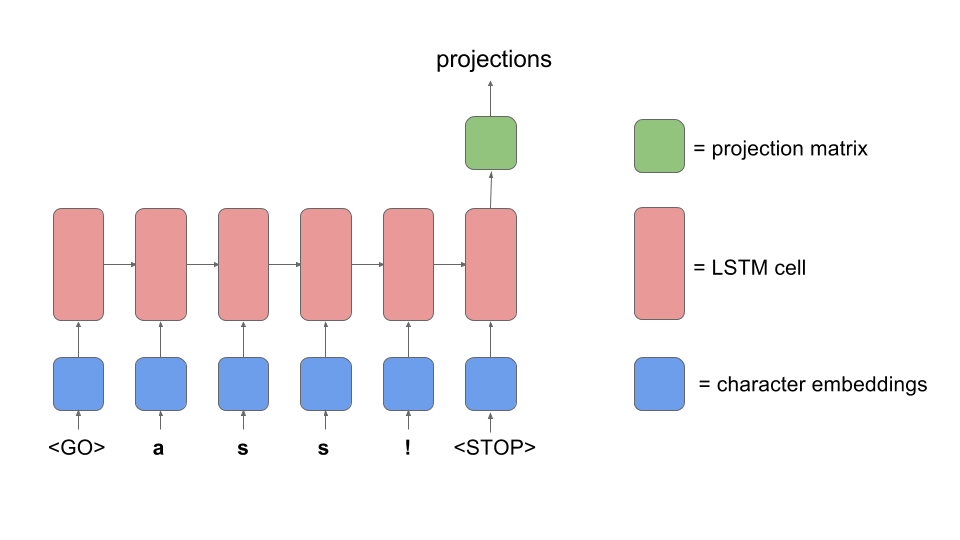
\includegraphics[width=15cm, height=8cm]{Network_Diagram.png}
\end{center}
\end{figure}
\vspace*{-1.3cm}
We used a character-level LSTM for our base recurrent model because of its ability to ``remember'' information throughout the comment. We used the tanh activation since ReLu with the LSTM led to numeric stability issues when gradients grew large. It also seems unnecessary to use ReLu activations since they are usually used for mitigating the vanishing gradient problem, a problem from which the LSTM was designed not to suffer. 

All the networks used softmax-cross-entropy loss after projection and, after some experimentation, Xavier initialization on the embedding and projection matrices. The hidden state used the default initializer uniformly randomly initializes every weight from the range $[-\frac{\sqrt{3}}{\sqrt{\text{dim}}}, \frac{\sqrt{3}}{\sqrt{\text{dim}}}]$

\subsubsection*{Bi-directional LSTM}
We also tried a bi-directional LSTM so that the network could combine information from both earlier and later in the comment in order to determine whether the comment was an insult. The bidirectional LSTM is just two copies of the diagram above except with tied word embeddings, and with a projection matrix twice as large in order to combine the two LSTMs. The second LSTM is also fed the comment in reverse.

We believe this network has a higher performance ceiling than does a single-directional RNN, but this dataset is not large enough to test that hypothesis. There is simply not enough data to train one, let alone two LSTMs. 

\subsubsection*{Multi-Layer LSTM}
A multi-layer LSTM stacks LSTMs on top of each other at each time step. Theoretically, this allows LSTMs to learn higher-level concepts (like words under character replacements). Deep networks are notoriously difficult to train, and they require a lot of data. We did not expect impressive performance from LSTMs on this dataset. 

\subsubsection*{Character GRU}
We also tried using a Gated Recurrent Unit (GRU) for comparison with the LSTM. The GRU has fewer gates than the LSTM, essentially only controlling whether to update stored information. In GRUs have been shown to benefit from ReLu activation, but We only used tanh activations because time constraints prevented us from retuning the hyperparameters for ReLu. We would be curious to see if GRUs perform better when using ReLu, but this will likely be a small difference compared to the gain from Yahoo's larger dataset. 

\subsection*{Regularization and Hyperparameter Search}
Neural networks have so many parameters that they easily overfit data. These models are also quite sensitive to the choice of hyperparameters, and in particular to learning rate. 

We searched for hyperparameters by obtaining a seed set of 40 randomly picked combinations of parameters within a ``best practices'' range. After running training all 40 models, we selected the best one and then did a greedy search by parameter over a large range of values. We first searched for learning rate, then character dropout, dropout, L2 regularization, and finally hidden state size. We experimented with changing the embedding size, but bigger was always better so we set it equal to the hidden state size. Selected charts of the greedy search are included in the appendix.


\subsection*{Evaluation}
Most of the prior literature evaluated their models with either Area Under the [ROC] Curve (AUC) or the F1 score. F1 is the better metric since AUC measures parts of the ROC curve in which we will never operate. On the other hand, F1 scores exist at each point on the curve and we are free to select the one which we care about the most. We chose a threshold of 0.5, though the threshold can be varied depending upon relative importance of precision versus recall. 

\textbf{AUC:}
The area under the ROC curve is called the AUC and is related to the Mann-Whitney U score. It roughly corresponds to the probability that a randomly picked insult will have a higher score than a randomly picked noninsult. 

This is a commonly used metric, and we included it so that our models could be compared to other results, however we believe it is not a good metric for this task. In addition to the problem discussed above, in insult detection we don't care whether a randomly selected pair has the right ordering - we want to make sure the insult has a score above the threshold and the noninsult doesn't. AUC is not a good proxy for this, as evidenced by the poor correlation between AUC and F1. 

\textbf{F1:}
F1 score weights the importance of precision versus recall.
It is defined as the harmonic mean of the two as follows:
$$ \textsc{F1} = \frac{\text{precision} \cdot \text{recall}}{\text{precision} + \text{recall}} $$

Precision and recall can be weighted in the calculation above although we gave them equal weights. Depending on the availability of moderators to handle false positives, or the danger of letting insults slip through, one may want to evaluate F1 with a different weighting. 


%%%%%%%%%%%%%%%%%%%%%%%%%%%%%%%%%%%%%%%%%%%%%%%%%%%%%%%%%%%%%%%%%%%%%%%%%%%%%%%%%
% 									RESULTS
%%%%%%%%%%%%%%%%%%%%%%%%%%%%%%%%%%%%%%%%%%%%%%%%%%%%%%%%%%%%%%%%%%%%%%%%%%%%%%%%%
\section*{Results}


\begin{table}[t]
\caption{Results}
\begin{center}
\begin{tabular}{l{5cm}P{1cm}P{1cm}}
\label{results}
\textbf{Model} & \textbf{F1 Score} & \textbf{AUC}\\
\hline \\
Unigrams                        & 0.663		& 0.794 \\ 
Uni + Bigrams                   & 0.640		& 0.794 \\ 
Stemming + Unigrams         		& 0.671		& 0.796 \\ 
Stemming + TFIDF + Unigrams     & 0.603		& 0.767 \\
Stemming + Uni + Bigrams        & 0.665		& \textbf{0.816} \\ 
Stem + 1,2grams SVM             & 0.580		& 0.736 \\
GloVe Vector-Avg 100d        		& 0.507		& 0.694 \\
GloVe Vector-Avg 200d      			& 0.568		& 0.733 \\
GloVe Vector-Avg 300d  					& 0.615		& 0.743 \\
charLSTM 50d										& 0.704	& 0.769 \\
charLSTM 300d        						& \textbf{0.721}	& 0.795 \\
bd charLSTM 300d        				& 0.702		& 0.756 \\
2-layer charLSTM 300d        		& 0.667		& 0.510 \\
GRU 300d 												& 0.694 	& 0.756
\end{tabular}
\end{center}
\end{table}

\subsection*{Comparison to Prior Work}
Table \ref{results} contains the experimental results. The baseline performance is quite similar to what prior work reports for hate speech on different datasets. Djuric et al. \cite{Djuric:2015:HSD:2740908.2742760} report a BOW AUC of 0.7889 while here BOW achieves 0.816. With TFIDF the AUC dropped to 0.6933 in Djuric et al. while here it drops to 0.767.

The F1 scores for BOW were also similar to Warner et al. \cite{warner2012detecting} where they had an F1 of 0.63, our best baseline was 0.67). This was encouraging and demonstrated that this dataset was viable and the models were a strong and accurate baseline.

The GloVe averaging results are extremely close to those of Nobata et al. \cite{DBLP:conf/www/NobataTTMC16} who find that averaging pretrained word vectors yields an F1 of 0.631. Here we find an F1 of 0.615. 


\subsection*{Recurrent Architectures}
Of the architectures tried, the vanilla char-LSTM with 300d worked the best, with the bidirectional architecture coming second. We believe this is because the size of the dataset favored simpler architectures. In addition, because of the limited timeframe for the project, we spent less time tuning these more interesting models. 

On the other hand, with a fixed architecture, bigger seems to be better. Large regularized models strongly overfit the training set (even with regularization!) but still achieve a higher F1 and AUC. See below, where performance on the validation set is plotted for various sized models.

\begin{figure}[H]
\label{size-matters}
\hspace*{-0.5cm}
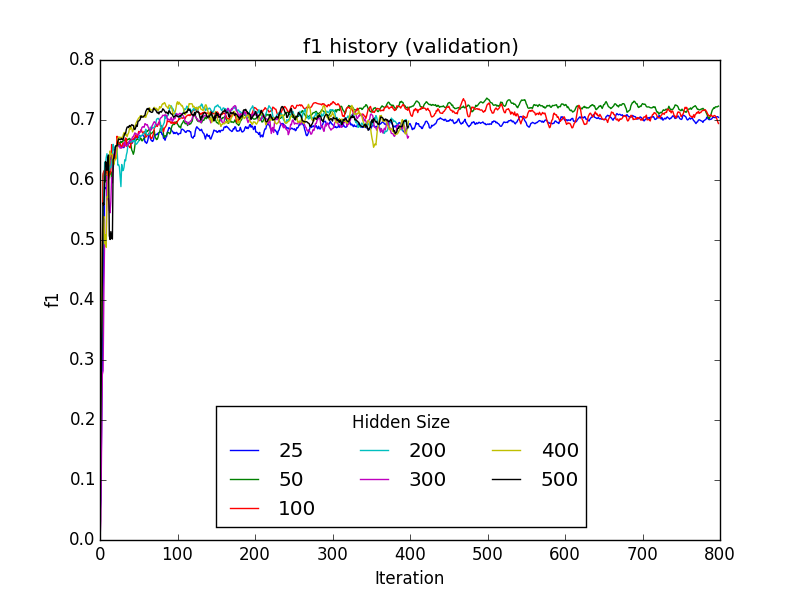
\includegraphics[width=7.5cm, height=5cm]{f1_history_validation_Hidden_Size.png}
\hspace*{-0.0cm}
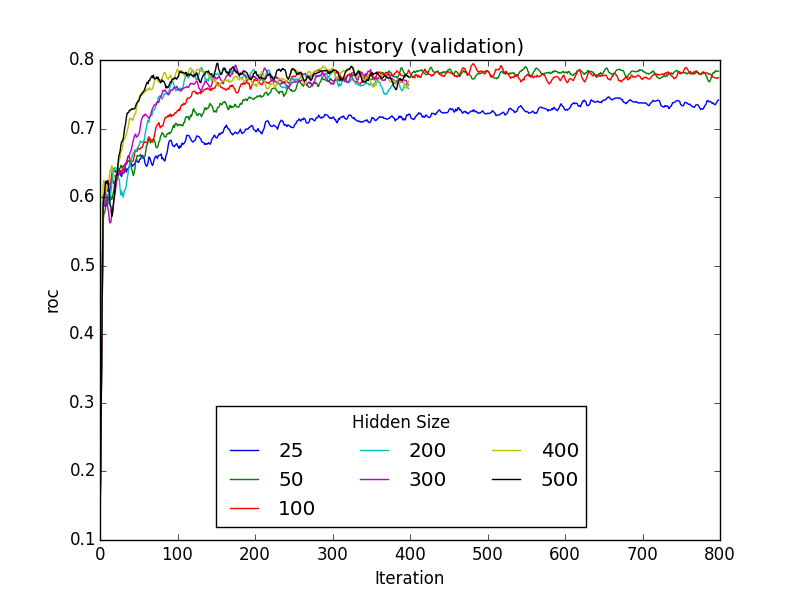
\includegraphics[width=7.5cm, height=5cm]{roc_history_validation_Hidden_Size.png}
\begin{center}
\caption{Performance of different sized models on validation set (5 epoch moving average). Large models were stopped after 400 epochs when performance began to decline.}
\end{center}
\end{figure}

\vspace*{-0.8cm}
Note also that there seems to be a strong ceiling for this architecture - all the sizes asymptotically approach a limiting F1 of around 0.72 and a limiting AUC of 0.8.

The small dataset made regularization extremely important for these models. Below are graphs for the char-LSTM without regularization (in blue) and with regularization (in green). Even with strong regularization, the cross entropy continues to increase on the validation set, but the F1 and AUC (``roc'' in the chart) is also higher. Increasing regularization beyond this local optimum does not help validation set performance and hampers the models ability to fit the training data (in red).

\begin{figure}[H]
\label{effect-regularization}
\hspace*{-0.5cm}
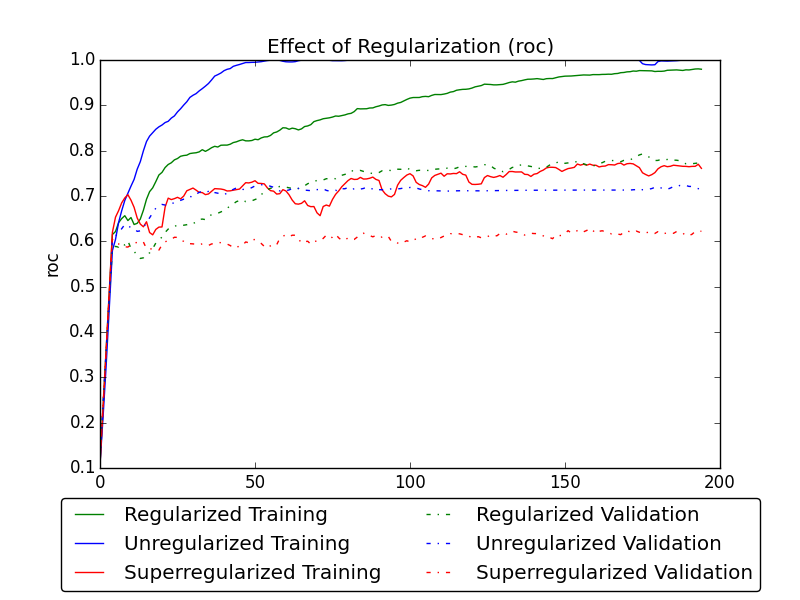
\includegraphics[width=7.5cm, height=5cm]{roc_train_v_valid_Effect_of_Regularization.png}
\hspace*{-0.0cm}
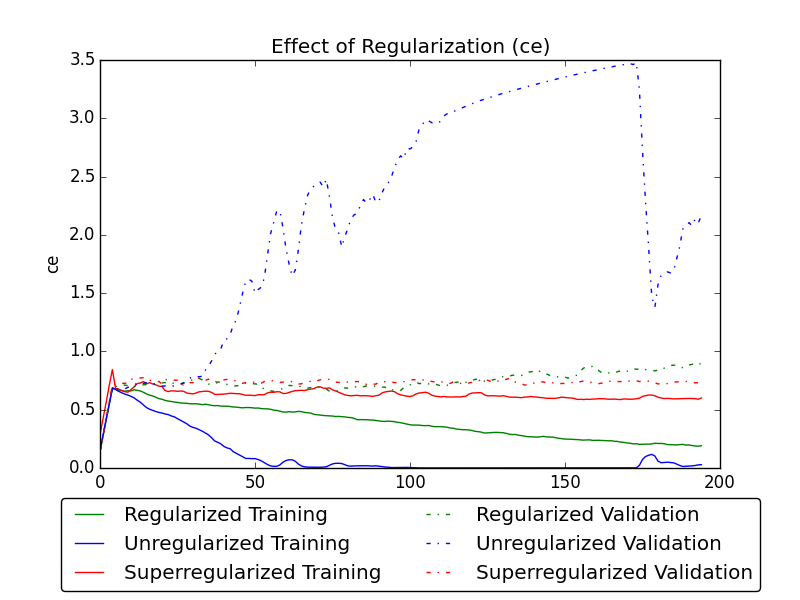
\includegraphics[width=7.5cm, height=5cm]{ce_train_v_valid_Effect_of_Regularization.png}
\end{figure}

As always, the best regularizer is more data, and we plan to run these models on the Yahoo data set when it is released. It will be interesting to see if it differentiates the recurrent models from linear ones. 

\section*{Analysis}
With only 5000 comments and 1250 insults, the dataset is quite small, so it is unsurprising that the linear models would do well compared to the neural models. However, it is surprising that unigrams had the best F1 score of the linear BOW models. These results agree with those of Warner et al. \cite{warner2012detecting} who trained on data from Yahoo and also data from the American Jewish Congress (and presumably have more than 5000 comments, though they only say that they have thousands of insults). This suggests that even such linear models need more data, that BOW does not work very well, or both.

For the recurrent models, character dropout proved to be particularly helpful, and we believe this is because the online comments were so noisy. Whether due to character dropout or just the character-level structure of the data, the model ended up learning suffixes. The figure below shows what the model would predict if the comment ended at each letter (and was followed by a STOP token).
\begin{figure}[H]
\begin{tabular}{llll}
\hspace*{0.1cm} {\color{bostonuniversityred} \textbf{f  u  c  k  e  r}} & 
\hspace*{1.0cm} {\color{bostonuniversityred} \textbf{s u c k e r}} & 
\hspace*{0.9cm} {\color{bostonuniversityred} \textbf{t r u c k e r}} & 
\hspace*{1.1cm} {\color{Ao} \textbf{l e v e r}} \\

\hspace*{-1cm} 

\includegraphics[width=3.5cm, height=0.5cm]{fucker.png}
& 
\includegraphics[width=3.5cm, height=0.5cm]{sucker.png}
& 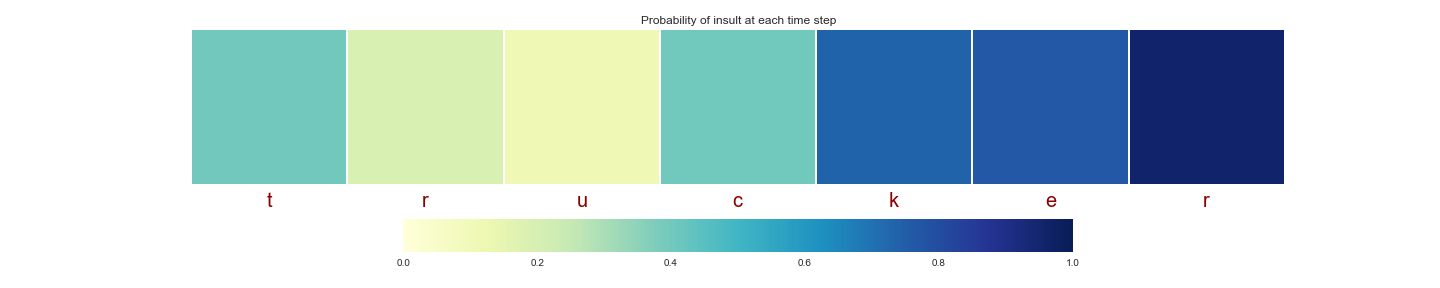
\includegraphics[width=3.5cm, height=0.5cm]{trucker.png}
& 
\includegraphics[width=3.5cm, height=0.5cm]{lever.png} \\
\end{tabular}
\caption{The char-LSTM seems to learn some suffixes (-cker) as well as profanity}
\end{figure}


\subsection*{Error Analysis}
\textbf{Repetition} \textit{(xxxxx you're stupid xxxxx)}: Once the LSTM finds a character or character-gram it feels strongly about, repeating this set will exaggerate the classification. This can be abused to slip an insult under the radar, or could flag noninsults. This could be solved by reducing lengthening of characters, though the character LSTM was supposed to eliminate the need for this.

\textbf{Negation} \textit{(You’re not a stupid git)}:
The character-LSTM does not handle negation, and seems to ignore negation words. This is something that is known to be difficult for sequential models, and one solution is a recursive network or dynamic memory network - models which build up knowledge from base chunks and are able to reevaluate knowledge at higher levels of abstraction. 

\textbf{Learns grams} (\textit{you're a great cook}):
The character-LSTM would, at least in some ways, appear to be a fancy character n-gram detector. Just as it detects suffixes above, so it looks for a phrase like \textit{you're a} and propogates that knowledge to the final time step. You can see below that as soon as the LSTM sees \textit{you're a} it flags the comment - despite what comes after. From the second image below, we can see the LSTM knows \textit{great cook} is not an insult (in fact the phrase was in the training data).

On the other hand, the model is not only an ngram detector. It looks for more than just keywords, because although it knows \textit{bitch} is an insult, it gives a very low score to \textit{a female dog is sometimes called a bitch} - so it is somehow capturing the mitigating context. This example may be a problem of too little data as the phrase \textit{you're a} instantly flags almost any comment as an insult. 

\begin{figure}[H]
\begin{tabular}{ll}
\hspace*{-1cm} 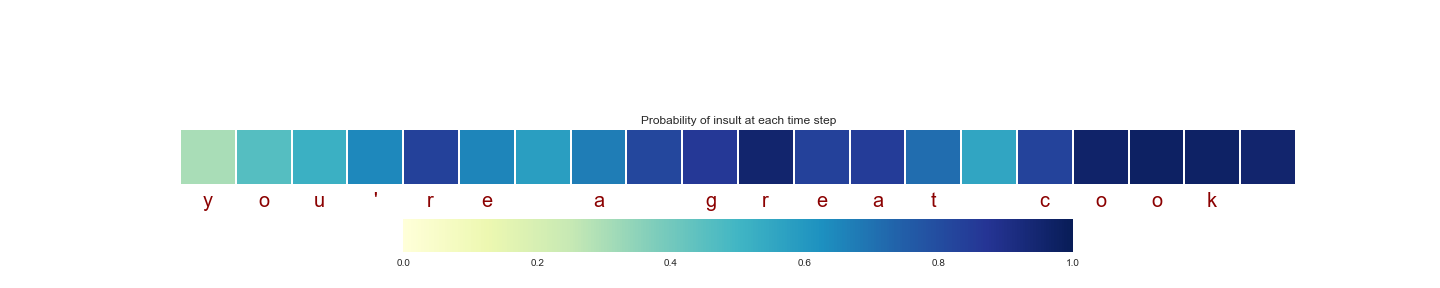
\includegraphics[width=8cm, height=2cm]{youre_a_great_cook.png} & 
\hspace*{-1cm} 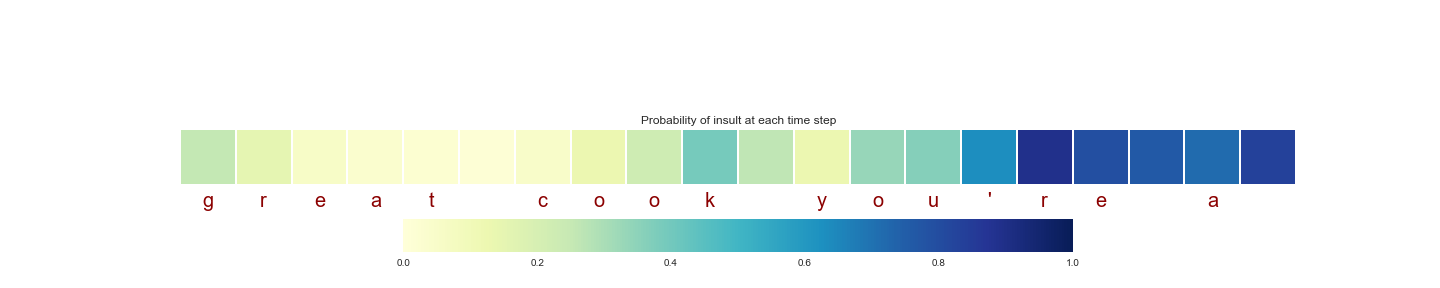
\includegraphics[width=8cm, height=2cm]{great_cook_youre_a.png} \\
\vspace*{-2.1cm} \\
\hspace*{1.6cm} {\color{bostonuniversityred} \textbf{you're a great cook }} & 
\hspace*{1.8cm} {\color{bostonuniversityred} \textbf{great cook you're a }}\\
\vspace*{0.6cm} \\ 
\end{tabular}
\caption{char-LSTM as word}
\end{figure}


\textbf{Dependencies on later parts of the comment} \textit{(``stupid'' would be a mean word to call you)}:
This is a tough concept for a unidirectional RNN to capture. The model would have to reevaluate its initial parse of \textit{stupid} (as a predicate adjective in \textit{[you are] stupid}, for example), and change it to a noun. A unidirectional RNN would have to have the different possible parses captured in the hidden state, and it is not clear that an LSTM learns to do this. A bidirectional RNN may be able to capture the same information by using the reversed LSTM, but the dataset is quite small for a bidirectional RNN to learn effectively.

\subsection*{Strength Analysis}
\textbf{Long distance dependencies} \textit{(you're dumb, but these characters should distract you from that fact!)}
Somewhat surprisingly, the model succeeds even when the insult comes at the beginning of the sentence. The filler words throw off the baseline models, but the char-RNN gets this right. This works even in the case where the filler words are a non-insult.

\textbf{Can handle obfuscations and OOV words} \textit{(GOF CKYOURSELF.)}
As a result of learning parts of words, the model often can correctly classify a comment when it contains out-of-vocabulary words that look similar to words it already knows. This is a large advantage over word-level models.


%%%%%%%%%%%%%%%%%%%%%%%%%%%%%%%%%%%%%%%%%%%%%%%%%%%%%%%%%%%%%%%%%%%%%%%%%%%%%%%%%
% 									CONCLUSION
%%%%%%%%%%%%%%%%%%%%%%%%%%%%%%%%%%%%%%%%%%%%%%%%%%%%%%%%%%%%%%%%%%%%%%%%%%%%%%%%%
\section*{Conclusions}
All character-level recurrent networks outperformed the baseline models in terms of F1 while underperforming the AUC values. Given the application of these networks, F1 is a more desirable criterion. In addition, character-rnns are more robust to techniques to evade detection, and the techniques that do work (lengthening) can be handled by appropriate preprocessing. 

Other problems inherent in the simple LSTM may be solved with a more powerful architecture like a tree-LSTM that could learn to build up meaning from characters and parts of words, rather than word tokens themselves. Such an architecture would better be able to handle negation and may better use information from throughout the comment (instead of just learning grams). 

These architectures are promising, but to truly test their effectiveness we will have to wait until more data is available, and this should be in the near future. 


\subsection*{Future Work}
When Yahoo's data becomes available, it will be interesting to see how bidirectional recursive architectures fare. We believe the gap between the baseline and the char-LSTM will increase as the amount of data increases.

We will also be interested to see which domains (comments in Yahoo! Finance vs Yahoo! Sports) are amenable to automatic detection methods. 

Finally, it will be interesting to see how well combined word and character-level models do, especially when combined with backoff. These models could combine information about words (for example, starting with pretrained vectors) when is available with character-level information for obfuscated or misspelled words. 

\newpage
\nocite{*}
\bibliographystyle{unsrt}
\bibliography{papers}

\newpage
\begin{appendices}
\textbf{Hyperparameter Search:} For brevity, only th charts for the more relevant dataset are included in the appendix. All charts are a 5-epoch moving average of the dependent variables.

\textbf{Learning Rate\footnote{Training is included to demonstrate ability to overfit.}: $0.001$}

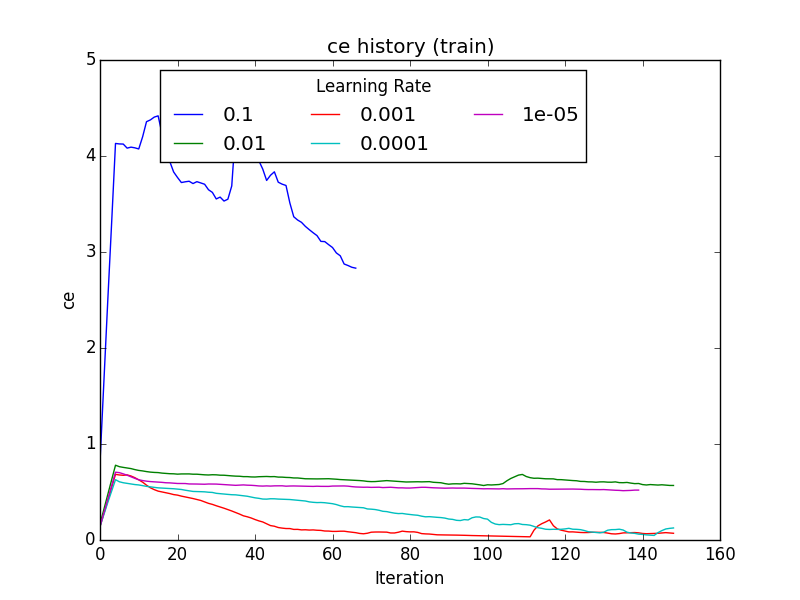
\includegraphics[width=4.5cm, height=3cm]{ce_history_train_Learning_Rate.png}
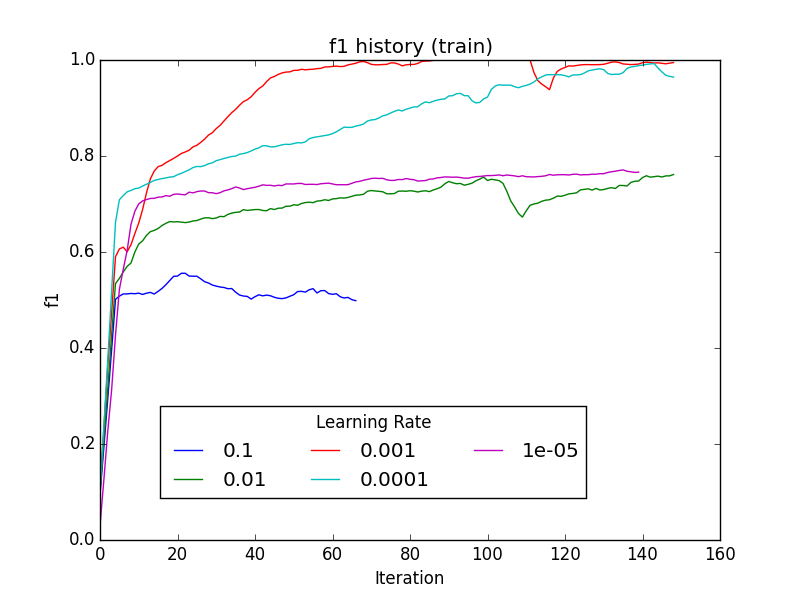
\includegraphics[width=4.5cm, height=3cm]{f1_history_train_Learning_Rate.png}
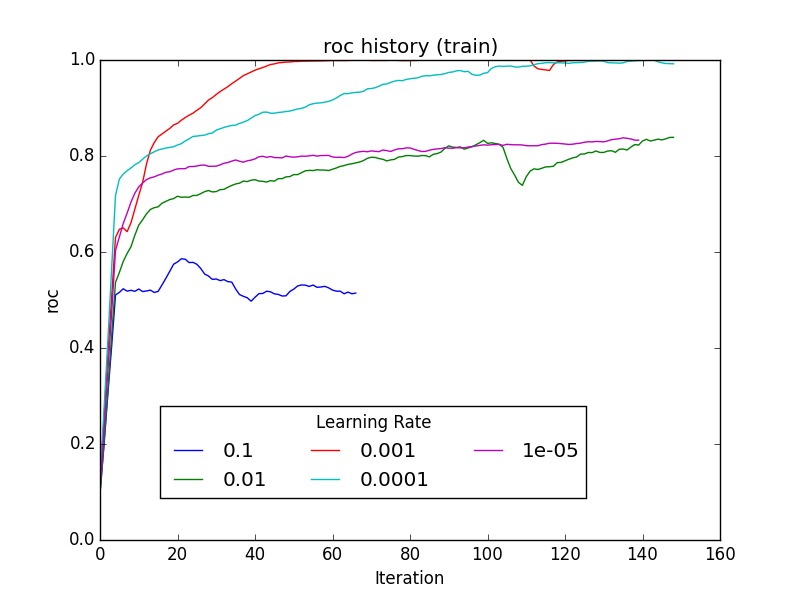
\includegraphics[width=4.5cm, height=3cm]{roc_history_train_Learning_Rate.png}

\textbf{Character Dropout: $30\%$}

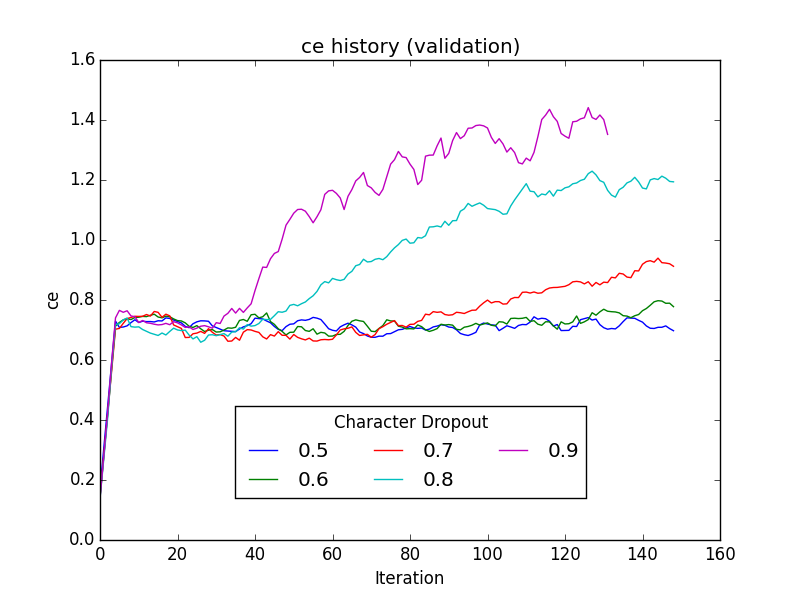
\includegraphics[width=4.5cm, height=3cm]{ce_history_validation_Character_Dropout.png}
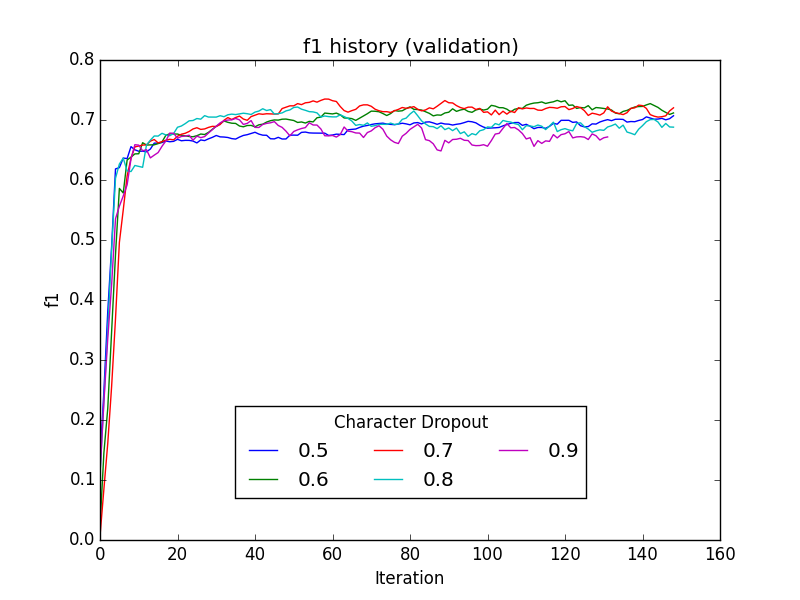
\includegraphics[width=4.5cm, height=3cm]{f1_history_validation_Character_Dropout.png}
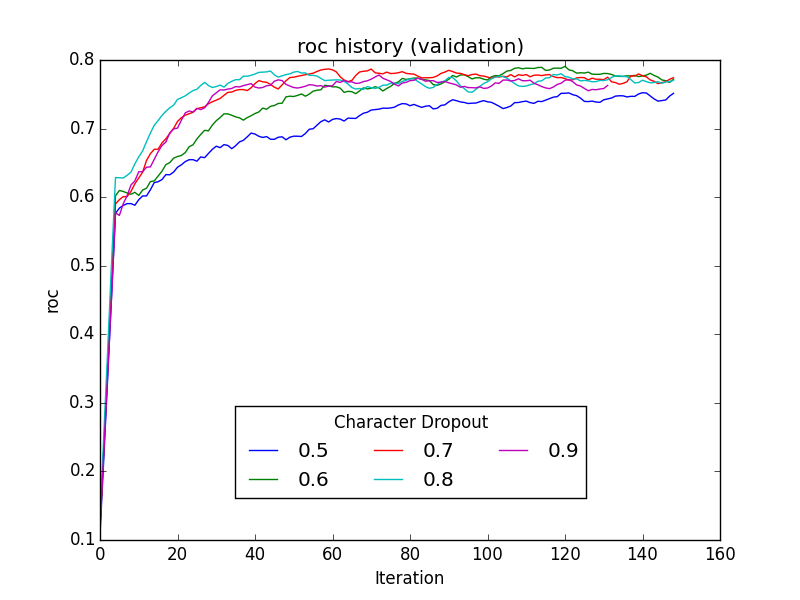
\includegraphics[width=4.5cm, height=3cm]{roc_history_validation_Character_Dropout.png}

\textbf{Dropout: $50\%$}

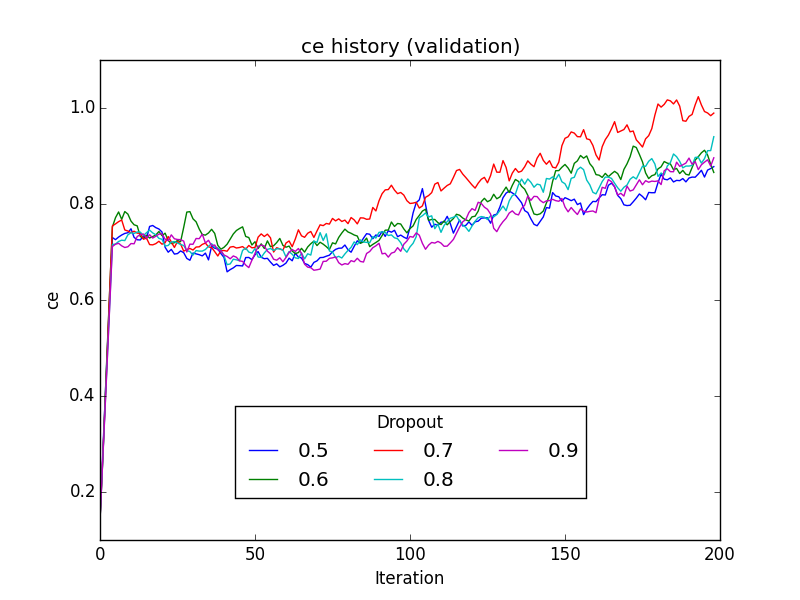
\includegraphics[width=4.5cm, height=3cm]{ce_history_validation_Dropout.png}
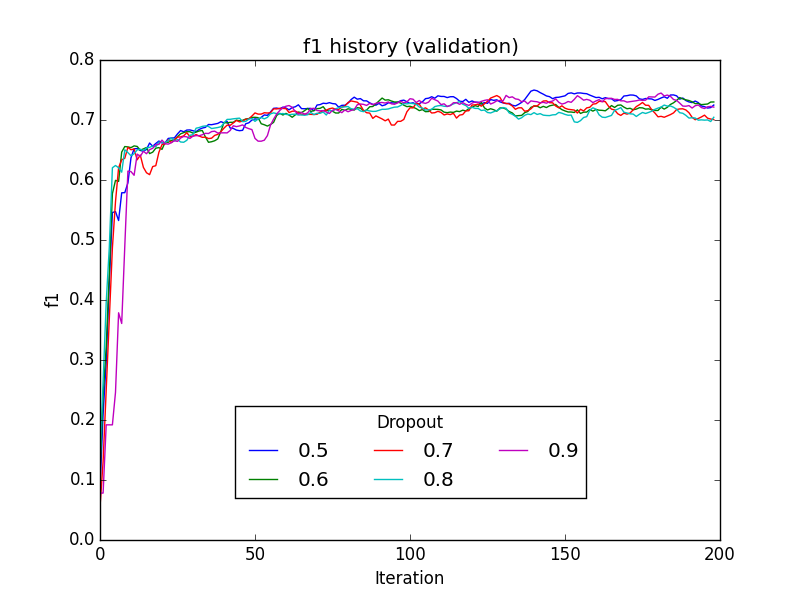
\includegraphics[width=4.5cm, height=3cm]{f1_history_validation_Dropout.png}
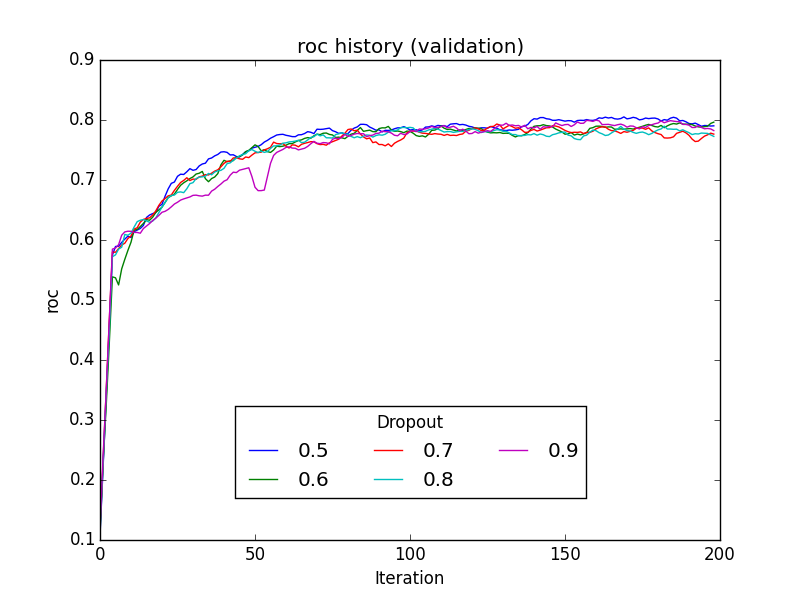
\includegraphics[width=4.5cm, height=3cm]{roc_history_validation_Dropout.png}

\textbf{L2 Regularization: $1e^{-6}$}

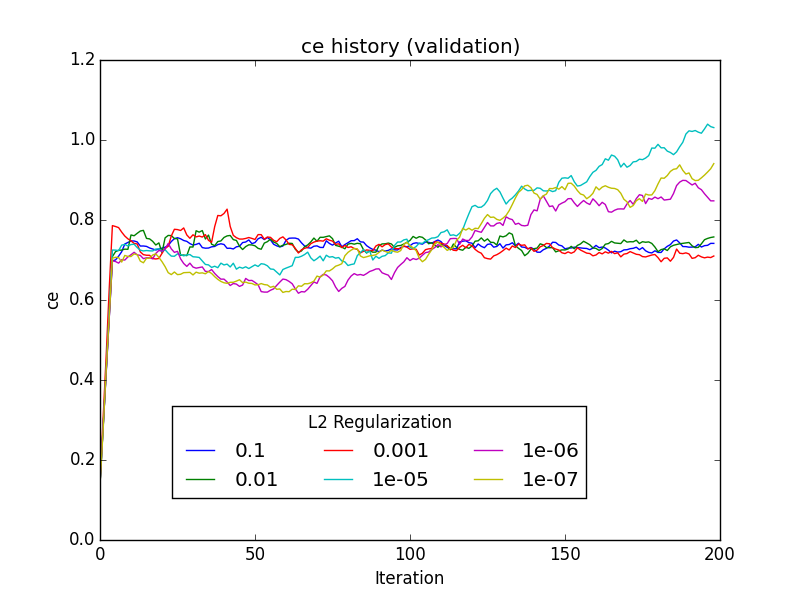
\includegraphics[width=4.5cm, height=3cm]{ce_history_validation_L2_Regularization.png}
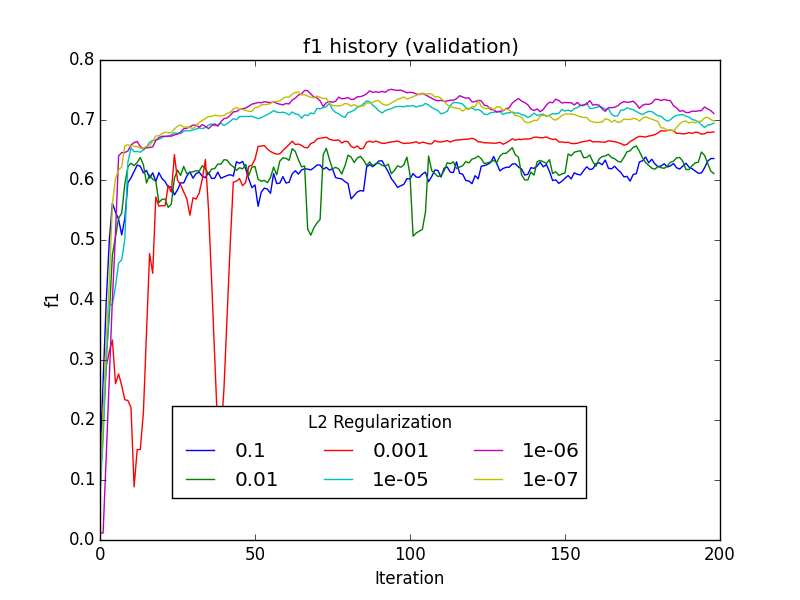
\includegraphics[width=4.5cm, height=3cm]{f1_history_validation_L2_Regularization.png}
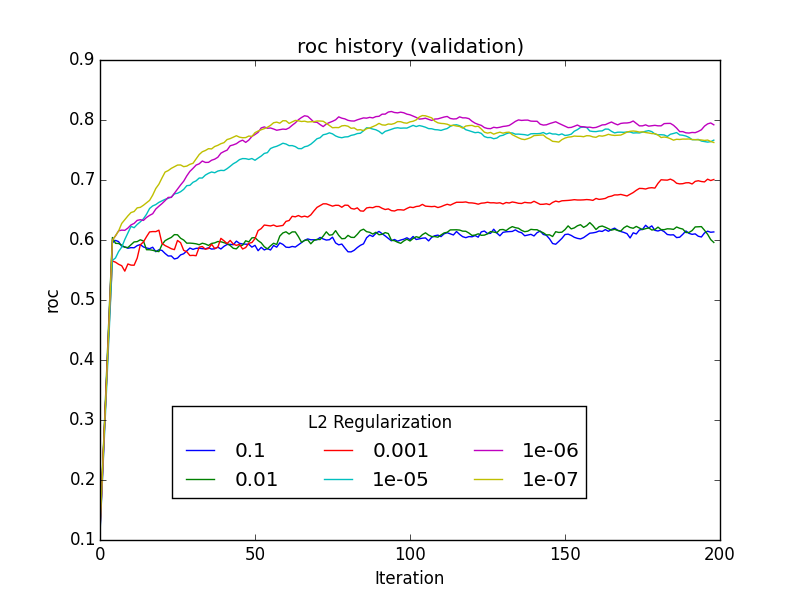
\includegraphics[width=4.5cm, height=3cm]{roc_history_validation_L2_Regularization.png}

\textbf{Hidden Dimension\footnote{Large networks were stopped early after they scores leveled off and validation error started increasing.}: $300$}

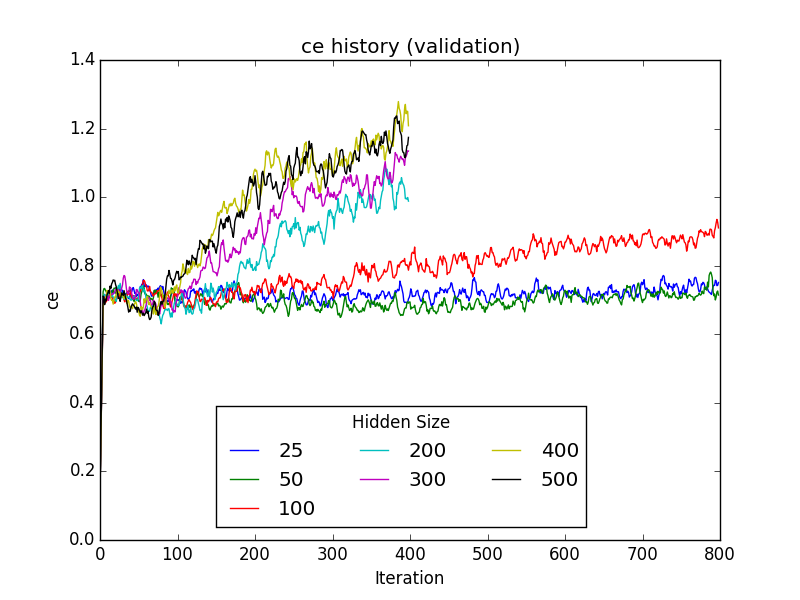
\includegraphics[width=4.5cm, height=3cm]{ce_history_validation_Hidden_Size.png}
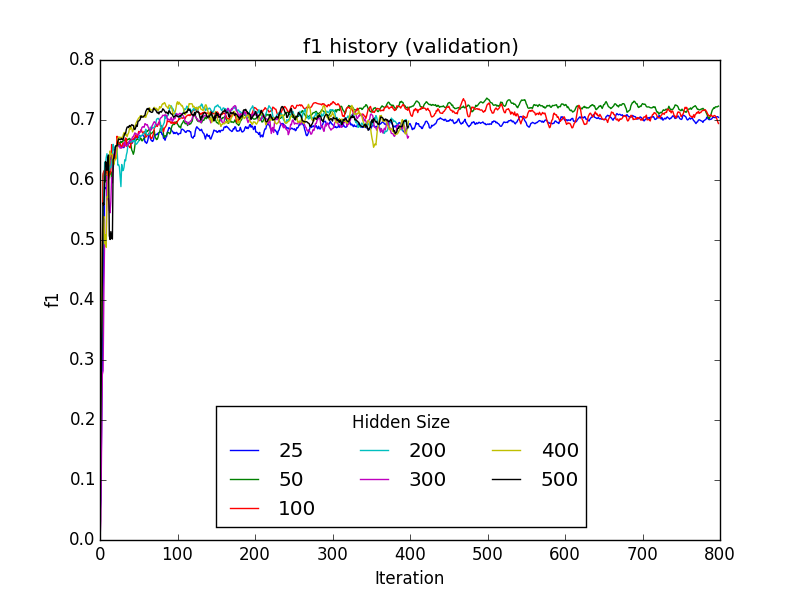
\includegraphics[width=4.5cm, height=3cm]{f1_history_validation_Hidden_Size.png}
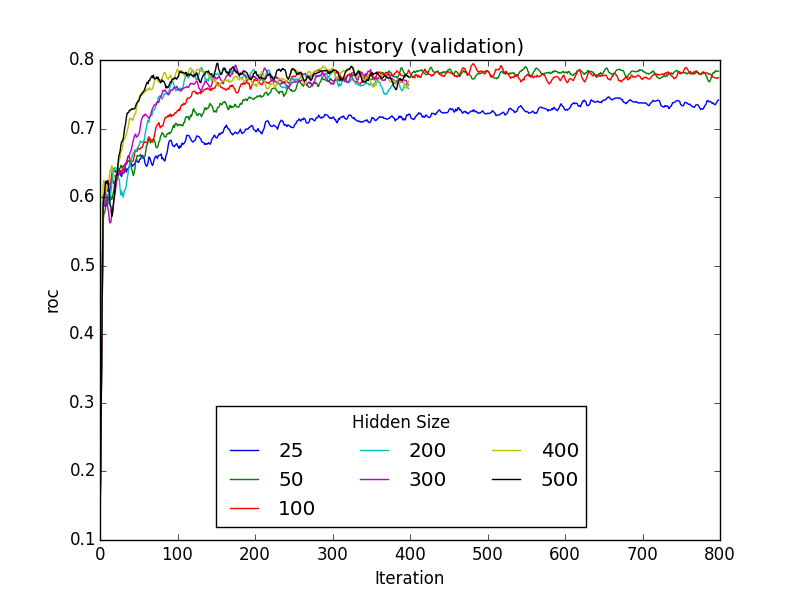
\includegraphics[width=4.5cm, height=3cm]{roc_history_validation_Hidden_Size.png}
\end{appendices}

\end{document}
